\documentclass[czech]{article}% use option titlepage to get the title on a page of its own.
\usepackage{booktabs}
\usepackage{indentfirst}
\usepackage{listings}
\usepackage{hyperref}
\usepackage{fancyhdr}
\usepackage{a4wide}
\usepackage{dblfloatfix}
\usepackage{float}
\usepackage{upgreek}
\usepackage{graphicx}
\usepackage[table,xcdraw]{xcolor}
\usepackage[czech]{babel}
\usepackage[autostyle=true,czech=quotes]{csquotes}

\renewcommand \thesection {\arabic{section}}
\renewcommand \thesubsection {\thesection.\alph{subsection}}
\renewcommand \thesubsubsection {\thesubsection.\alph{subsubsection}}

\title{Pravděpodobnost a statistika\\
    \large Domácí úkoly 1S-4S\\
    \large Zadání 123}

\author{Martin Pustka} 
\date{\today}

\setlength{\headheight}{12.41254pt}
\pagestyle{fancy}
\fancyhf{}
\lhead{Martin Pustka, PUS0065}
\rhead{Číslo zadání 123}
\chead{Ostrava, AR 2020/2021}
\cfoot{\thepage}

\restylefloat{table}
\restylefloat{figure}

\begin{document}

\maketitle

\noindent
Jméno studenta: Martin Pustka\\
Osobní číslo: PUS0065\\
Jméno cvičícího: Ing. Michal Béreš\\

\begin{table*}[!b]
    \centering
    \begin{tabular}{|l|p{5cm}|p{3cm}|}
        \hline
        & Datum odevzdání & Hodnocení \\
        \hline
        Domácí úkol 1: & 9. duben 2021 & 5/5 \\
        \hline
        Domácí úkol 2: & 30. duben 2021 & 2.5/5\\
        \hline
        Domácí úkol 3: & 7. května 2021 & 5/5\\
        \hline
        Domácí úkol 4: & 14. května 2021& \\
        \hline
        Celkem: & & \\
        \hline
    \end{tabular}
\end{table*}
\newpage
\tableofcontents
\newpage

\noindent
\textbf{Popis datového souboru}
\\\\
\noindent
Běžné zářivky trpí efektem pomalého nabíhání, tedy plného výkonu dosáhnou až po jisté době provozu. Toto chování je ovlivněno okolní teplotou, což v praxi znamená, že v chladném prostředí může zářivkám trvat výrazně déle než dosáhnou maximálního výkonu. 
\\\\
\noindent
Pro test náběhu zářivek na plný světelný výkon bylo vybráno celkem 350 zářivek od čtyř různých výrobců (Amber, Bright, Clear, Dim). Všechny zářivky měly deklarovaný maximální světelný tok 1000 lm. U každé zářivky byl změřen světelný tok po 30 sekundách od zapnutí, nejprve při teplotě 22 °C a poté při teplotě 5°C.
\\\\
\noindent
V souboru ukol\_X.xslx jsou pro každou z testovaných zářivek uvedeny následující údaje:
\begin{itemize}
    \item pořadové číslo zářivky,
    \item výrobce – Amber (A), Bright (B), Clear (C), Dim (D),
    \item naměřený světelný tok v lumenech při okolní teplotě 5°C,
    \item naměřený světelný tok v lumenech při okolní teplotě 22°C.
\end{itemize}

\noindent
\textbf{Obecné pokyny:}
\begin{itemize}
    \item Úkoly zpracujte dle obecně známých typografických pravidel.
    \item Všechny tabulky i obrázky musí být opatřeny titulkem.
    \item Do úkolů nevkládejte tabulky a obrázky, na něž se v doprovodném textu nebudete odkazovat.
    \item Bude-li to potřeba, citujte zdroje dle mezinárodně platné citační normy ČSN ISO 690.
\end{itemize}


\newpage
\section{Úkol 1S}
\subsection{Zadání}
Pomocí nástrojů explorační analýzy analyzujte světelný tok zářivek výrobce Amber po 30 sekundách od zapnutí při teplotách 5°C a 22°C. Data vhodně graficky prezentujte (krabicový graf, histogram, q-q graf) a doplňte následující tabulky a text.

Výsledky popisné statistiky lze vidět v tabulce \ref{tab:statAmber} a na obrazcích \ref{fig:Boxploty},\ref{fig:Histogram5},\ref{fig:Histogram22},\ref{fig:QQ5} a \ref{fig:QQ22}.
Boxplot obsahuje odlehlá pozorování, ostatní grafy jsou bez odlehlých pozorování.

\subsection{Tabulkové řešení}
\noindent
\begin{table}[H]
	\centering
	\caption{Světelný tok (lm) zářivek Amber v závislosti na teplotě (souhrnné statistiky)}
	\label{tab:statAmber}
	\begin{tabular}{lccl|cc}
        \hline
        \rowcolor[HTML]{F2F2F2} 
        \multicolumn{2}{l}{\cellcolor[HTML]{F2F2F2}Světelný tok zářivek Amber (lm)} & & & \multicolumn{2}{l}{\cellcolor[HTML]{F2F2F2}Po   odstranění odlehlých pozorování} \\
        \rowcolor[HTML]{F2F2F2} 
        \hline
        & 5°C             & 22°C             && 5°C                                    & 22°C                                    \\
        \hline
        rozsah souboru           & 71                          & 71                           &  & 70                                     & 71                                   \\
        minimum                  & 750,0                       & 755,8                        &  & 750,0                                  & 755,8                                   \\
        dolní kvartil            & 774,0                       & 774,0                        &  & 773,4                                  & 774,0                                   \\
        medián                   & 797,8                       & 801,9                        &  & 797,4                                  & 801,9                                   \\
        průměr                   & 797,5                       & 797,6                        &  & 795,6                                  & 797,6                                   \\
        horní kvartil            & 818,3                       & 819,6                        &  & 817,9                                  & 819,6                                   \\
        maximum                  & 927,4                       & 875,1                        &  & 882,9                                  & 875,1                                   \\
        směrodatná odchylka      & 30,5                        & 25,8                         &  & 26,4                                   & 25,8                                    \\
        variační koeficient (\%) & 3,8                         & 3,2                          &  & 3,3                                    & 3,2                                     \\
        šikmost                  & 1,2                         & 0,1                          &  & 0,3                                    & 0,1                                     \\
        špičatost                & 3,4                         & -0,5                         &  & 0,0                                    & -0,5                                    \\
        \hline
        \rowcolor[HTML]{F2F2F2} 
        \multicolumn{3}{l}{\cellcolor[HTML]{F2F2F2}Identifikace   odlehlých pozorování – vnitřní hradby}                 &&   &                                         \\
        \hline
        dolní mez                & 707,6                       & 705,6                        &  & 706,6                                  & 705,6                                   \\
        horní mez                & 884,7                       & 888,0                        &  & 884,6                                  & 888,0                                   \\
        \hline
    \end{tabular}
\end{table}

\newpage
\subsection{Grafické řešení}

\begin{figure}[H]
	\centering
	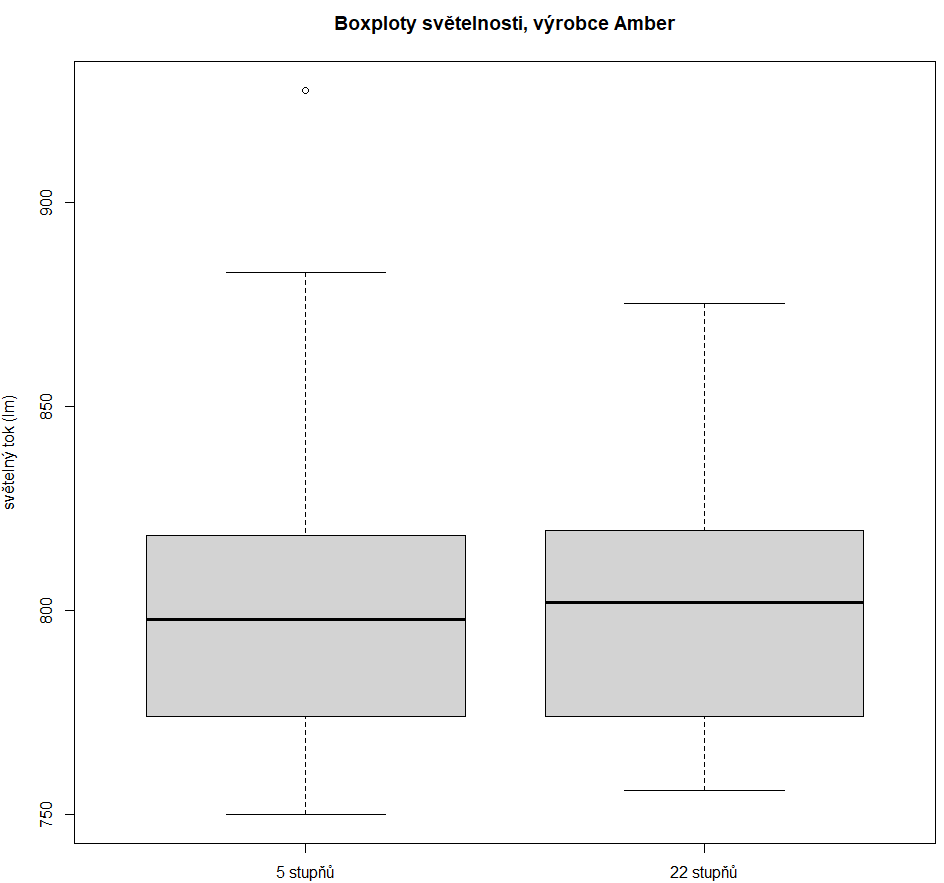
\includegraphics[width=0.6\textwidth]{Figures/Boxploty.png}
	\caption[Boxploty světelnosti, Amber]{Boxploty světelnosti, Amber}
	\label{fig:Boxploty}
\end{figure}

\newpage
\begin{figure}[H]
	\centering
	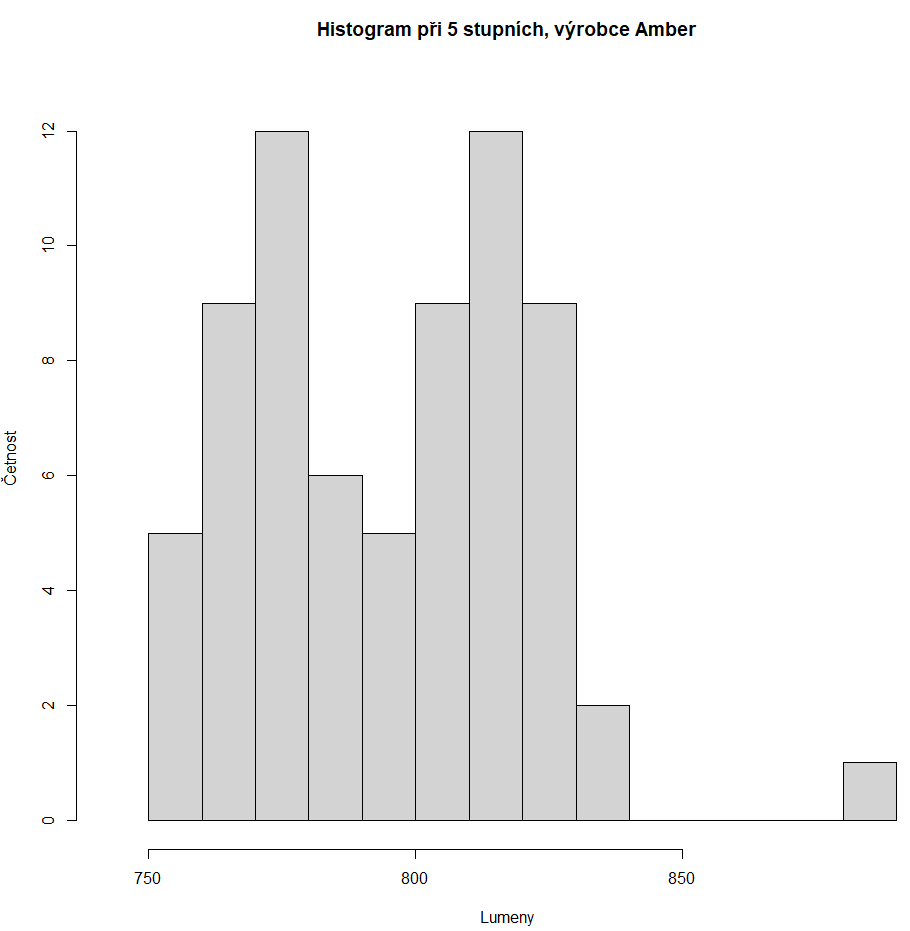
\includegraphics[width=0.6\textwidth]{Figures/Histogram5.png}
	\caption[Histogram světelnosti 5C, Amber]{Histogram světelnosti při 5 stupních, výrobce Amber}
	\label{fig:Histogram5}
\end{figure}

\begin{figure}[H]
	\centering
	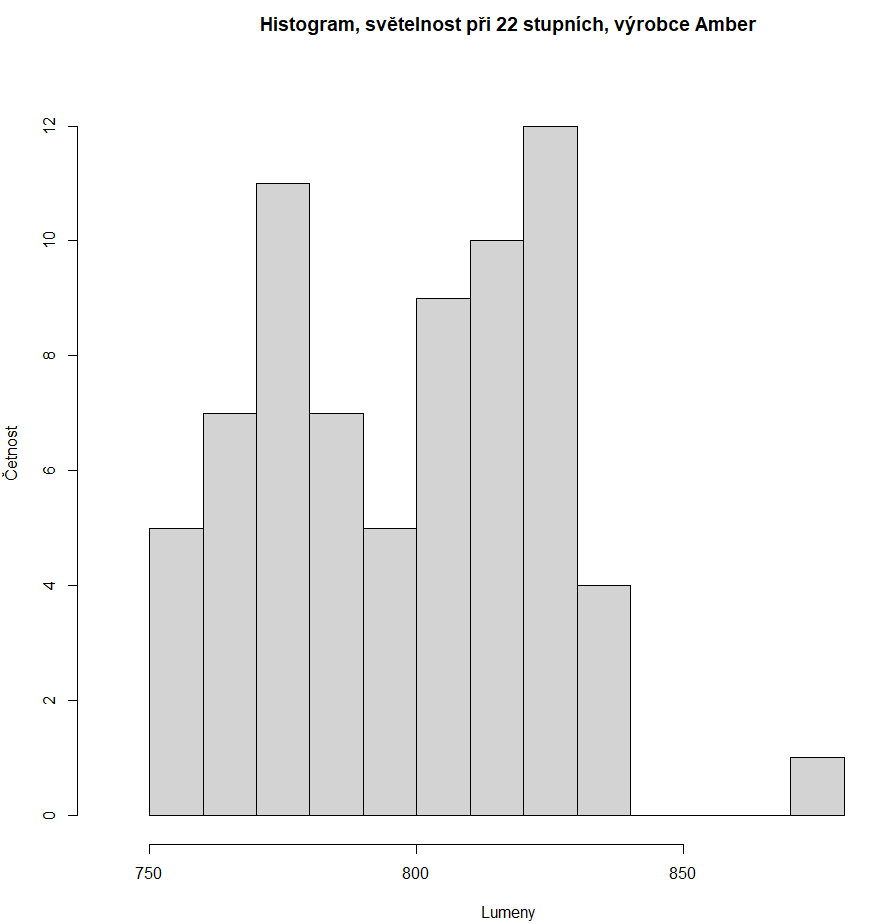
\includegraphics[width=0.6\textwidth]{Figures/Histogram22.png}
	\caption[Histogram světelnosti 22C, Amber]{Histogram světelnosti při 22 stupních, výrobce Amber}
	\label{fig:Histogram22}
\end{figure}

\newpage
\begin{figure}[H]
	\centering
	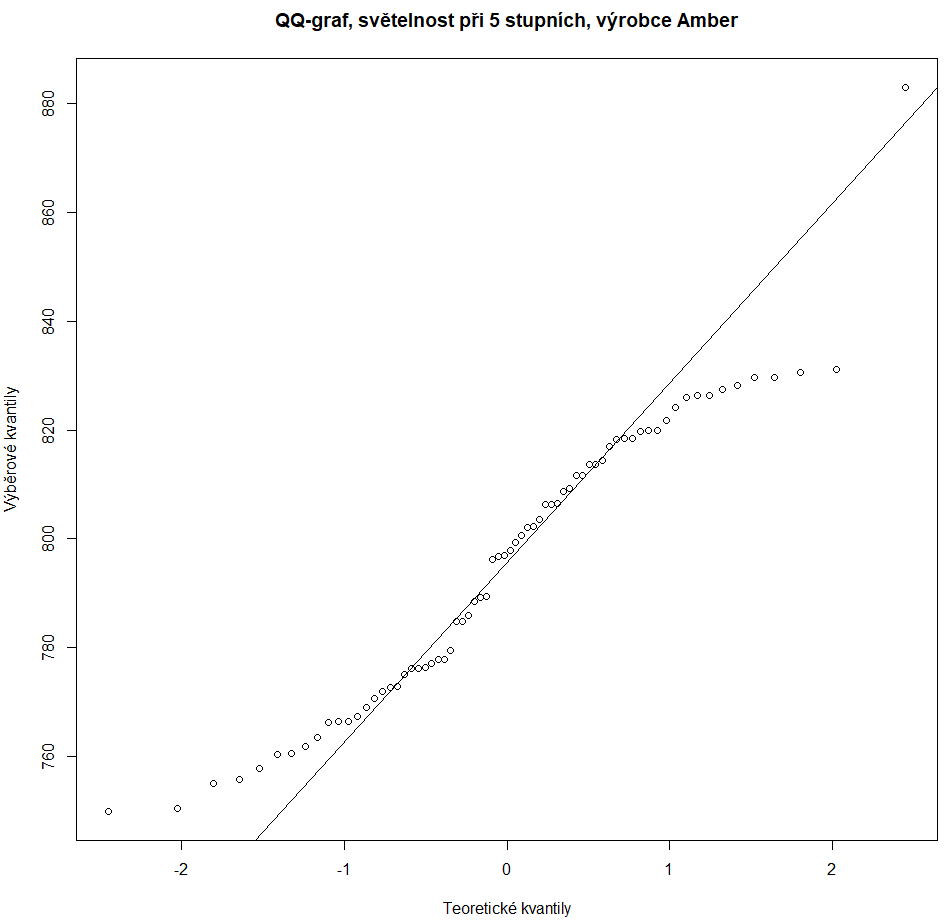
\includegraphics[width=0.6\textwidth]{Figures/QQ5.png}
	\caption[QQ graf světelnosti 5C, Amber]{QQ graf světelnosti při 5 stupních, výrobce Amber}
	\label{fig:QQ5}
\end{figure}

\begin{figure}[H]
	\centering
	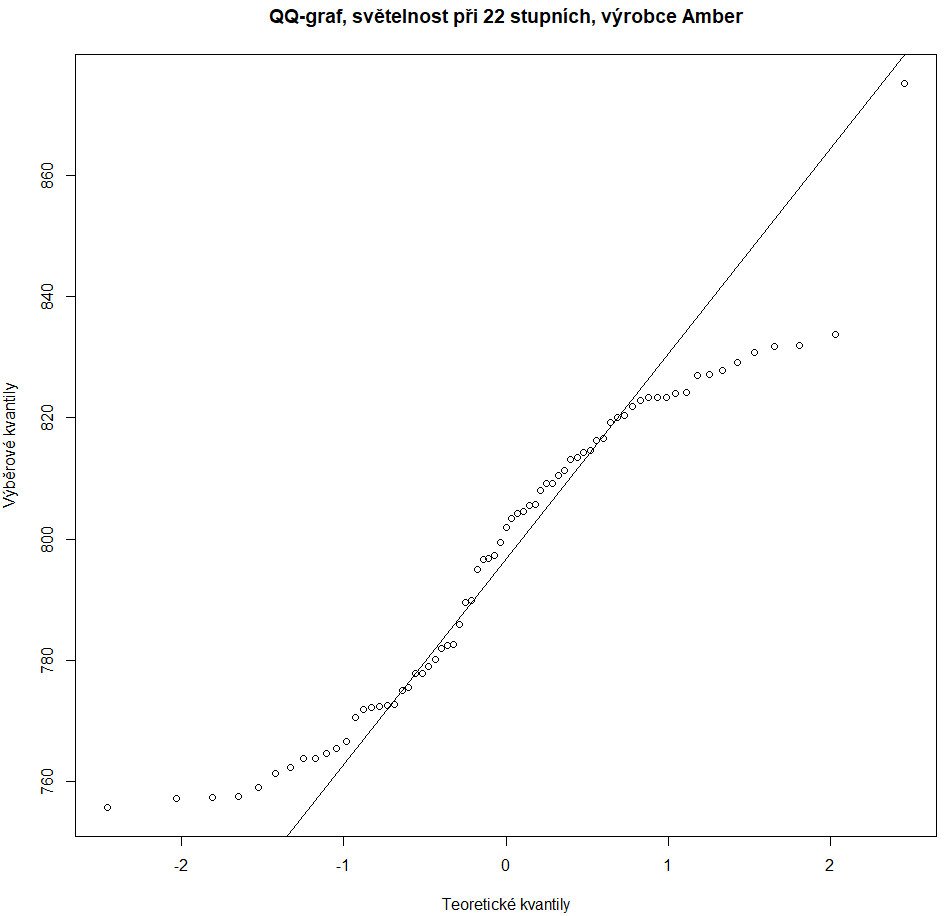
\includegraphics[width=0.6\textwidth]{Figures/QQ22.png}
	\caption[QQ graf světelnosti 5C, Amber]{QQ graf světelnosti při 5 stupních, výrobce Amber}
	\label{fig:QQ22}
\end{figure}

\newpage
\subsection{Textové řešení}

\textbf{Analýza světelného toku zářivek výrobce Amber (po 30 sekundách od zapnutí, při teplotě 5°C)}

Během testu byl měřen světelný tok \textit{71} kusů zářivek výrobce Amber. 
Naměřená světelný tok při teplotě 5°C se pohyboval v rozmezí \textit{750,0} lm až \textit{927,4} lm. 
Světelný tok zářivek č. \textit{27} byl na základě metody vnitřních hradeb identifikován jako 
odlehlé pozorování a nebude zahrnut do dalšího zpracování. Možné příčiny vzniku odlehlých pozorování jsou: \textit{chyby v měření nebo při výrobě}. 
Dále uvedené výsledky tedy pocházejí z analýzy světelný toku \textit{70} kusů zářivek. Jejich průměrný světelný tok byl \textit{795,6} lm, 
směrodatná odchylka pak \textit{26,4} lm. U poloviny testovaných zářivek světelný tok nepřekročil \textit{797,4} lm. 
V polovině měření se světelný tok pohyboval v rozmezí \textit{773,4} lm až \textit{817,9} lm. 
Vzhledem k hodnotě variačního koeficientu (\textit{3,3 \%}) lze analyzovaný soubor považovat za homogenní.\\


\textbf{Analýza světelného toku zářivek výrobce Amber (po 30 sekundách od zapnutí, při teplotě 22°C)}

Během testu byl měřen světelný tok \textit{71} kusů zářivek výrobce Amber. 
Naměřená světelný tok při teplotě 22°C se pohyboval v rozmezí \textit{755,8} lm až \textit{875,1} lm. 
Žádné z měření nebylo identifikováno jako odlehlé pozorování. 
Dále uvedené výsledky tedy pocházejí z analýzy světelný toku \textit{71} kusů zářivek. Jejich průměrný světelný tok byl \textit{797,6} lm, 
směrodatná odchylka pak \textit{25,8} lm. U poloviny testovaných zářivek světelný tok nepřekročil \textit{801,9} lm. 
V polovině měření se světelný tok pohyboval v rozmezí  \textit{774,0} lm až \textit{819,6} lm. 
Vzhledem k hodnotě variačního koeficientu (\textit{3,2} \%) lze analyzovaný soubor považovat za homogenní.\\


\textbf{Ověření normality světelného toku zářivek výrobce Amber po 30 sekundách od zapnutí při teplotě 5°C na základě explorační analýzy}

Na základě grafického zobrazení (viz obrázek \ref{fig:QQ5}) a výběrové šikmosti a špičatosti (výběrová šikmost i špičatost leží v intervalu (-2;2)) 
lze předpokládat, že světelný tok zářivek výrobce Amber při teplotě 5°C má normální rozdělení. Dle pravidla 3$\upsigma$ 
lze tedy očekávat, že přibližně 95 \% zářivek bude mít světelný tok v rozmezí \textit{742,9} lm až \textit{848,3} lm.\\


\textbf{Ověření normality světelného toku zářivek výrobce Amber po 30 sekundách od zapnutí při teplotě 22°C na základě explorační analýzy}

Na základě grafického zobrazení (viz obrázek \ref{fig:QQ22}) a výběrové šikmosti a špičatosti (výběrová šikmost i špičatost leží v intervalu (-2;2)) 
lze předpokládat, že světelný tok zářivek výrobce Amber při teplotě 22°C má normální rozdělení. Dle pravidla 3$\upsigma$ 
lze tedy očekávat, že přibližně 95 \% zářivek bude mít světelný tok v rozmezí \textit{746,0} lm až \textit{849,2} lm.\\


\newpage
\section{Úkol 2S}
Porovnejte pokles světelného toku po 30 sekundách od zapnutí při snížení okolní teploty z 22°C 
na 5°C u zářivek od výrobců Amber a Bright. Nezapomeňte, že použité metody mohou vyžadovat 
splnění určitých předpokladů. Pokud tomu tak bude, okomentujte splnění/nesplnění těchto předpokladů 
jak na základě explorační analýzy (např. s odkazem na histogram apod.), tak exaktně pomocí metod statistické indukce.


% A)
\subsection{}
Graficky prezentujte srovnání poklesů světelného toku zářivek výrobců Amber a Bright 
při snížení okolní teploty (vícenásobný krabicový graf, histogramy, q-q grafy). 
Srovnání okomentujte (včetně informace o případné manipulaci sdatovým souborem).

\begin{figure}[H]
	\centering
	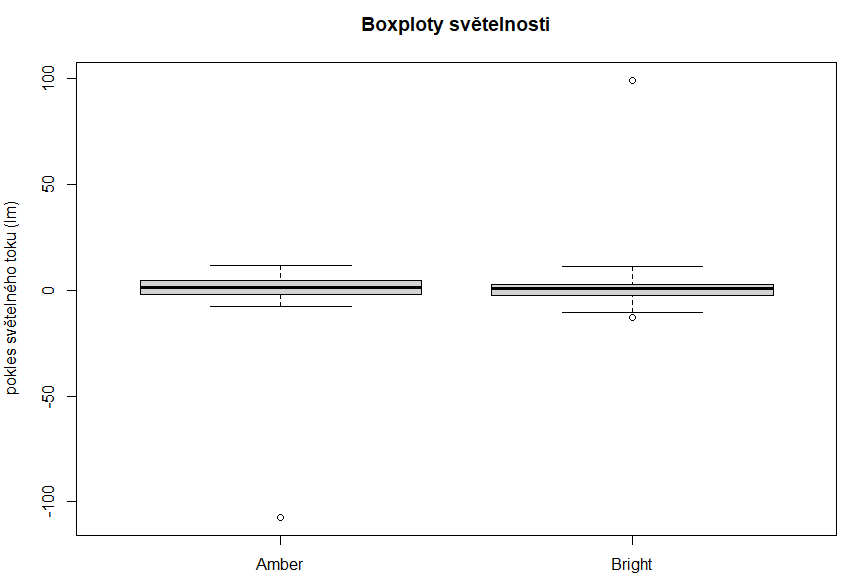
\includegraphics[width=0.9\textwidth]{Figures/Boxploty_2.png}
	\caption[Boxploty světelnosti, Amber a Bright]{Boxploty světelnosti, Amber a Bright}
	\label{fig:Boxplot2}
\end{figure}

U obou výrobců byly pozorovány 3 odlehlé pozorování (viz Obr. \ref{fig:Boxplot2}), tyto jsme se rozhodli z dálšího zpracování vypustit. 
Podle vizualizace srovnání poklesů světelného toku zářivek výrobců Amber a Bright (viz Obr. \ref{fig:Boxplot2}), Obr. \ref{fig:QQaHist_2})) lze usoudit, že k výraznému poklesu 
světelnéhu toku při snížení okolní teploty nedošlo.

\begin{figure}[H]
	\centering
	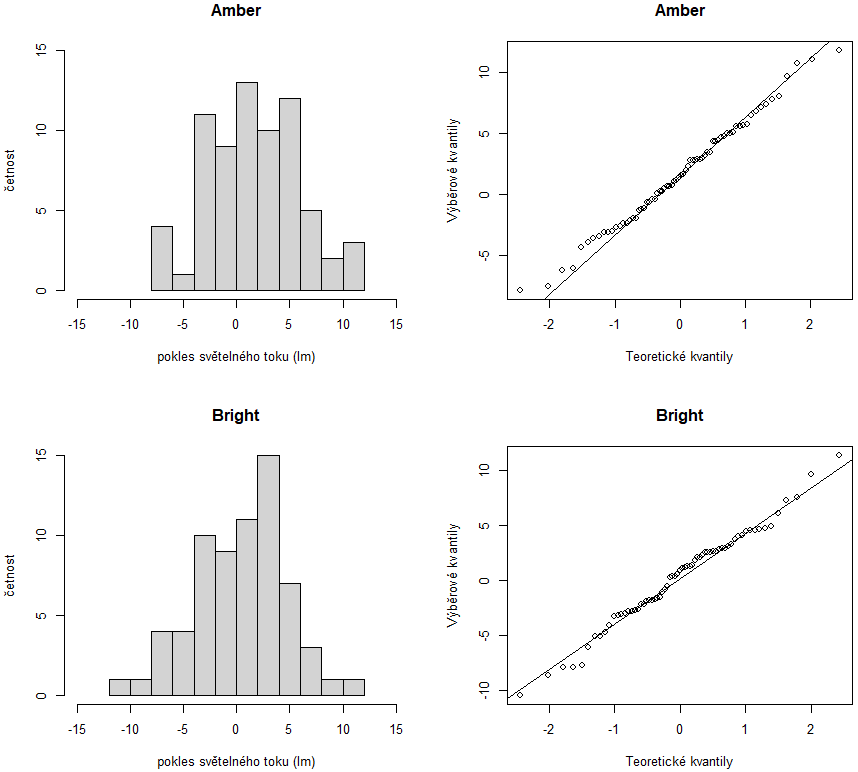
\includegraphics[width=0.9\textwidth]{Figures/QQaHistogram_2.png}
	\caption[Histogramy a Q-Q grafy světelnosti]{Histogramy a Q-Q grafy světelnosti, Amber a Bright, odstraněná pozorování}
	\label{fig:QQaHist_2}
\end{figure}


% B)
\newpage
\subsection{}
Na hladině významnosti 5 \% rozhodněte, zda jsou střední poklesy (popř. mediány poklesů) 
světelného tokuzářivek výrobců Amber a Bright statisticky významné. 
K řešení využijte bodové a intervalové odhady i testování hypotéz. Výsledky okomentujte.

Dle prezentovaných Q-Q grafů (viz Obr. \ref{fig:QQaHist_2}) lze usuzovat, že poklesy světelného toku zářivek u výrobce Amber i výrobce Bright 
lze modelovat normálním rozdělením. Šikmost i špičatost (viz Tab. \ref{tab:normSymet_2}) odpovídají normálnímu rozdělení.

\begin{table}[H]
	\centering
	\caption{Ověření normality poklesu světelného toku zářivek}
	\label{tab:normSymet_2}
    \begin{tabular}{c|c|c|c|c}
        & šikmost & stand. špičatost & \begin{tabular}[c]{@{}c@{}}Shapirův-Wilkův test\\ (p-hodnota)\end{tabular} & \begin{tabular}[c]{@{}c@{}}Test symetrie \\(p-hodnota)\end{tabular} \\
        \hline
        výrobce Amber  & 0,1    & -0,4            & 0,872                                                       & 0,681 \\
        \hline
        výrobce Bright & -0,1   & 0,1             & 0,646                                                       & 0,110 \\
    \end{tabular}
\end{table}

Dle Shapirova-Wilkova testu lze na hladině významnosti 0,05 pokles světelného toku zářivek 
u výrobce Amber i u výrobe Bright modelovat normálním rozdělením (viz Tab. \ref{tab:normSymet_2}).

Rozdělení poklesů světelných toků zářivek lze u výrobce Amber i u výrobce Bright považovat za 
symetrické. (viz šikmosti, výsledky testu symetrie (Tab. \ref{tab:normSymet_2}) a tvar histogramů (Obr. \ref{fig:QQaHist_2})), 
proto lze pro intervalové odhady a test významnosti stř. hodnot v případě obou výrobců použít Studentův t-test.

Vzhledem k tomu, že očekáváme poklesy světelností (s klesající teplotou se 
světelný tok zářivek snižuje), volíme levostranné intervalové odhady / levostranné testy.

Střední hodnotu poklesu světelnosti zářivek výrobce Bright očekáváme při teplotě 5 °C na cca 1,67 lm. 
95\% levostranný intervalový odhad stř. hodnot poklesu světelného toku zářivek výrobce Amber je (0,78;$\infty$) lm.
Intervalový odhad, stejně jako p-hodnota, ukazují, že stř. hodnota poklesu světelnosti je statisticky významně větší než nula. 
Tj. na hladině významnosti 0,05 lze pokles světelného toku žárovek výrobce Amber považovat za statisticky významný (viz Tab. \ref{tab:odhady}). 

Střední hodnotu poklesu světelnosti zářivek výrobce Bright očekáváme při teplotě 5 °C na cca 0,27 lm. 
95\% levostranný intervalový odhad stř. hodnot poklesu světelného toku zářivek výrobce Bright je (-0,62;$\infty$) lm.
Intervalový odhad, stejně jako p-hodnota, ukazují, že stř. hodnota poklesu světelnosti je statisticky významně větší než nula. 
Tj. na hladině významnosti 0,05 nelze pokles světelného toku žárovek výrobce Bright považovat za statisticky významný (viz Tab. \ref{tab:odhady}). 

\begin{table}[H]
	\centering
	\caption{Odhad stř. hodnoty a test významnosti poklesu světelných toků zářivek (lm) dle výrobce}
	\label{tab:odhady}
    \begin{tabular}{c|c|c|c}
        & \begin{tabular}[c]{@{}c@{}}bodový odhad\\ (lm)\end{tabular} & \begin{tabular}[c]{@{}c@{}}95\% levostranný\\ intervalový odhad\\ (lm)\end{tabular} & \begin{tabular}[c]{@{}c@{}}Studentův \\ levostranný t-test\\ (p-hodnota)\end{tabular} \\
        \hline
        výrobce Amber  & 1,67                                                        & (0,78;$\infty$)                                                                                & 0,001                                                     \\
        \hline
        výrobce Bright & 0,27                                                        & (-0,62;$\infty$)                                                                               & 0,308                                                                 \\
    \end{tabular}
\end{table}


% C)
\newpage
\subsection{}
Na hladině významnosti 5\% rozhodněte, zda je rozdíl středních hodnot (mediánů) 
poklesů světelných toků zářivek výrobců Amber a Bright (při snížení okolní teploty) statisticky významný.
K řešení využijte bodový a intervalový odhad i čistý test významnosti. Výsledky okomentujte.

Vzhledem k potvrzení normality u výrobce Amber i Bright je třeba zjistit zda mezi rozptyly výrobců panuje shoda.

Na základě výsledku F-testu (viz Tab. \ref{tab:dvouvyberTest}) lze rozhodnout o shodě rozptylů (homoskedasticitě) a použít 
Dvouvýběrový Studentův t-test pro test stř. hodnot.

U zářivek výrobce Amber lze očekávat pokles ve světelném toku o cca 1,4 lm větší než u výrobce Bright. 
Odpovídající 95\% levostranný intervalový odhad tohoto rozdílu je (0,63;1,68) lm.
Intervalový odhad, stejně jako Dvouvýběrový Studentův t-test (viz Tab. \ref{tab:dvouvyberTest}) ukazují, že stř. hodnota 
poklesu světelného toku zářivek výrobce Amber není statistiky významně vyšší než u výrobce Bright.

\begin{table}[H]
	\centering
	\caption{Srovnání středních hodnot poklesu světelných toků zářivek (lm) výrobce Amber a Bright}
	\label{tab:dvouvyberTest}
    \begin{tabular}{c|c}
        Bodový odhad $\mu^A$ - $\mu^B$ (lm)                                   & 1,40        \\
        \hline
        F-test (p-hodnota)                                                    & 0,889        \\
        \hline
        95\% oboustranný intervalový odhad $\mu^A$ - $\mu^B$ (lm)             & (-0,08;2,88)  \\
        \hline
        Dvouvýběrový Studentův t-test (p-hodnota)                             & 1,000         \\
    \end{tabular}
\end{table}

\newpage
\section{Úkol 3S}
Na hladině významnosti 5 \% rozhodněte, zda se světelný tok zářivek při teplotě 5 °C liší 
v závislosti na tom, od kterého výrobce pocházejí. 
Posouzení proveďte nejprve na základě explorační analýzy a následně pomocí 
vhodného statistického testu, včetně ověření potřebných předpokladů. 
V případě, že se světelný tok zářivek jednotlivých výrobců statisticky významně liší, 
určete pořadí výrobců dle středního světelného toku (popř. mediánu světelného toku) zářivek při 5°C.

% A)
\subsection{}
Daný problém vhodným způsobem graficky prezentujte (vícenásobný krabicový graf, histogramy, q-q grafy). 
Srovnání okomentujte (včetně informace o případné manipulaci s datovým souborem).

U všech výrobců byla pozorována odlehlá pozorování, celkem 6 (viz Obr. \ref{fig:Boxplot3}), která byla z dalšího zpracování odstraněna.
Z histogramů a Q-Q grafů (viz Obr. \ref{fig:QQaHist_3}) nelze, mezi výrobci, pozorovat významné rozdíly mezi světelnostmi jejich zářivek.

\begin{figure}[H]
	\centering
	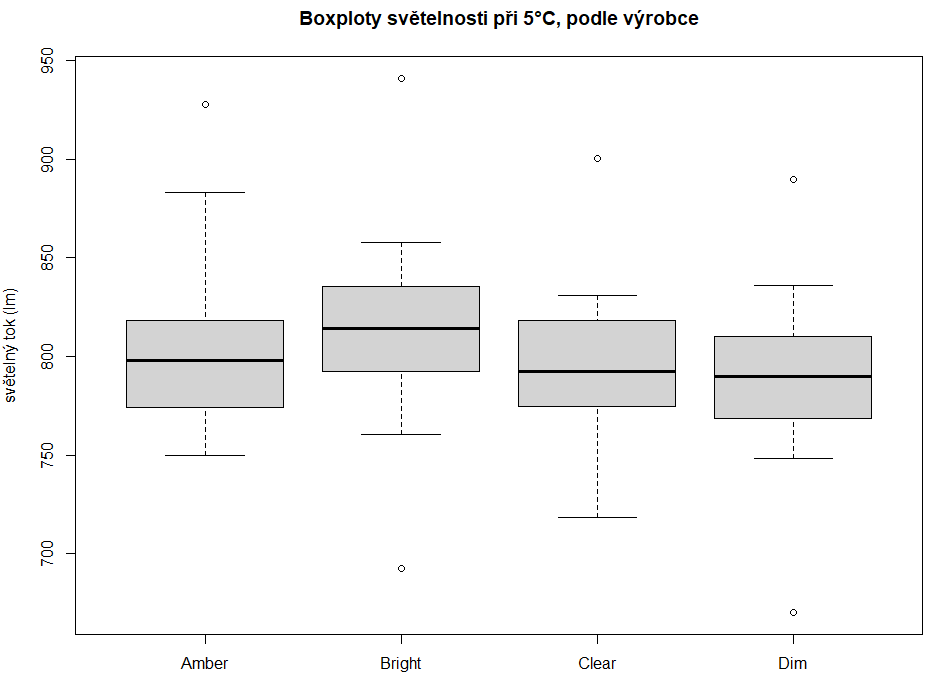
\includegraphics[width=0.9\textwidth]{Figures/Boxploty_3.png}
	\caption{Boxploty světelnosti při 5°C. Výrobce Amber, Bright, Clear a Dim}
	\label{fig:Boxplot3}
\end{figure}


\begin{figure}[H]
	\centering
	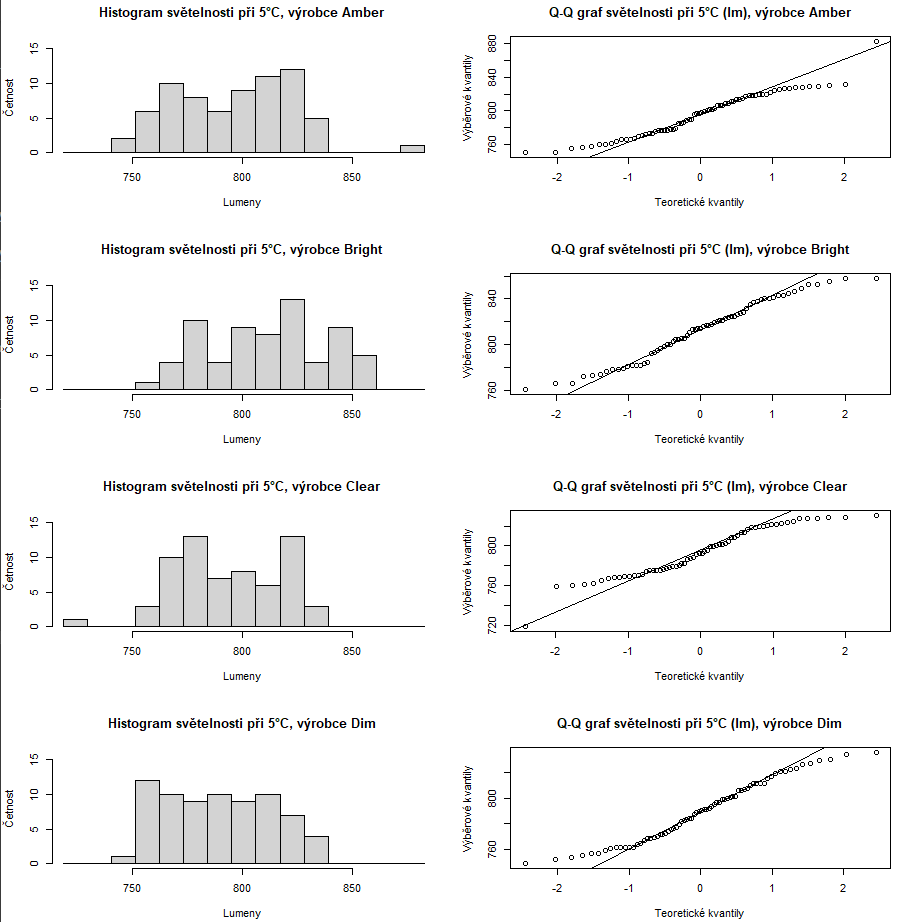
\includegraphics[width=0.9\textwidth]{Figures/QQaHistogram_3.png}
	\caption{Histogramy a Q-Q grafy světelnosti při 5°C. Výrobci Amber, Bright, Clear a Dim, odstraněná pozorování}
	\label{fig:QQaHist_3}
\end{figure}


% B)
\newpage
\subsection{}
Ověřte normalitu a symetrii světelného toku zářivek při teplotě 5°C u všech čtyř výrobců (empiricky i exaktně).

Podle prezentovaných grafů (viz Obr. \ref{fig:QQaHist_3}) nelze usuzovat, že světelný tok při 5 stupních je normálním rozdělením.

Šikmost i špičatost (viz Tab. \ref{tab:normSymet_3}) normálnímu rozdělení odpovídá, 
ale Shapirův-Wilkův test normalitu zamítl u všech výrobců s vyjímkou Bright.

Podle tvaru histogramů (viz Obr. \ref{fig:QQaHist_3}), výsledků šikmostí a výsledků testu 
symetrie (viz Tab. \ref{tab:normSymet_3}) lze u všech výrobců světelnost zářivek při 5°C považovat za symetrickou.

\begin{table}[H]
	\centering
	\caption{Srovnání normality a symetrie poklesu světelného toku zářivek, podle výrobce}
	\label{tab:normSymet_3}
    \begin{tabular}{c|c|c|c|c}
        Výrobce & Šikmost & Špičatost & \begin{tabular}[c]{@{}c@{}}Shapirův-Wilkův test \\ (p-hodnota)\end{tabular} & \begin{tabular}[c]{@{}c@{}}Test symetrie \\ (p-hodnota)\end{tabular} \\
        \hline
        Amber   & 0,3     & 0,0       & 0,009                                                                       & 0,477                     \\
        \hline
        Bright  & -0,1    & -1,0      & 0,079                                                                       & 0,448                     \\
        \hline
        Clear   & -0,3    & -0,3      & 0,005                                                                       & 0,638                     \\
        \hline
        Dim     & 0,1     & -1,1      & 0,031                                                                       & 0,823                     \\
    \end{tabular}
\end{table}

% C)
\newpage
\subsection{}
Ověřte homoskedasticitu (shodu rozptylů) světelného toku zářivek při teplotě 5 °C jednotlivých výrobců (empiricky i exaktně).

Podle Obr. \ref{fig:QQaHist_3} a poměru největšího a nejmenšího rozptylu světelností 
(viz Tab. \ref{tab:rozptyl_3}), $S_{A}^2/S_{D}^2 = 1,23$, se zdá, že srovnávané rozptyly lze považovat za srovnatelné.

Na základě Leveneho testu (p-hodnota = 0,781) nezamítáme předpoklad o shodě rozptylů.

\begin{table}[H]
	\centering
	\caption{Srovnání rozptylů světelnosti zářivek při 5°C, podle výrobce}
	\label{tab:rozptyl_3}
    \begin{tabular}{c|c}
        Výrobce & Rozptyl \\
        \hline
        Amber   & 694,9   \\
        \hline
        Bright  & 684,3   \\
        \hline
        Clear   & 582,5   \\
        \hline
        Dim     & 564,8   \\
    \end{tabular}
\end{table}


% D)
\newpage
\subsection{}
Určete bodové a 95\% intervalové odhady střední hodnoty (popř. mediánu) 
světelného toku zářivek při teplotě 5°C pro všechny srovnávané výrobce. 
(Nezapomeňte na ověření předpokladů pro použití příslušných intervalových odhadů.)

Předpoklad o symetrii rozdělení nelze zamítnout (viz Tab. \ref{tab:normSymet_3}).
Vzhledem k zamítnutí předpokladu o normálním rozdělení je pro srovnání mediánu použit Kruskalův-Wallisův test.

Pro výpočet bodového odhadu jsou použity mediány a pro výpočet 95\% intervalového odhadu Wilcoxnův test.

\begin{table}[H]
	\centering
	\caption{Odhad mediánů světelnosti zářivek při 5°C, podle výrobce}
	\label{tab:mediany_3}
    \begin{tabular}{c|c|c}
        Výrobce & Bodový odhad (lm) & 95\% intervalový odhad (lm) \\
        \hline
        Amber   & 797,4             & (789,1 ; 801,5)             \\
        \hline
        Bright  & 814,2             & (805,5 ; 819,5)             \\
        \hline
        Clear   & 792,2             & (787,6 ; 799,6)             \\
        \hline
        Dim     & 790,0             & (783,3 ; 795,3)             \\
    \end{tabular}
\end{table}

% u mediánu lze napsat, že očekáváme polovinu hodnot menších než 797,4..
Medián světelnosti zářivek výrobce Amber očekáváme při teplotě 5 °C na cca 797,4 lm. 
95\% intervalový odhad tohoto mediánu je (789,1 ; 801,5) lm. Výsledky výrobců Bright, Clear a Dim
lze interpretovat obdobně. Výrobce Bright poskytuje při 5°C vyšší světelnost o přibližně 20 lumenů než ostatní výrobci.
Výrobci Amber, Clear a Dim se v tomto parametru liší v řádu jednotek lumenů.

% E)
\newpage
\subsection{}
Čistým testem významnosti ověřte, zda je pozorovaný rozdíl středních hodnot 
(popř. mediánů) světelného toku zářivek při teplotě 5°C statisticky významný 
na hladině významnosti 5 \%. Pokud ano, zjistěte, zda lze některé skupiny výrobců 
označit (z hlediska světelného toku zářivek po 30 sekundách od zapnutí, při teplotě 5°C) 
za homogenní, tj. určete pořadí výrobců dle středních hodnot (popř. mediánů) 
světelného toku zářivek při 5°C. (Nezapomeňte na ověření předpokladů pro použití zvoleného testu.)

Na hladině významnosti 0,05 zamítám hypotézu o shodě mediánů (Kruskalův-Wallisův test, p-hodnota \textless{}\textless{}0,001), 
tj. mediány světelnosti při teplotě 5°C se významně liší mezi výrobci.

\begin{table}[H]
	\centering
	\caption{Dunnová post hoc analýza}
	\label{tab:dunn_3}
    \begin{tabular}{c|c|c|c|c}
        Výrobce & Amber & Bright    & Clear & Dim                           \\
        \hline
        Amber   & x     & 0,002     & 1,000 & 1,000                         \\
        \hline
        Bright  &       & x         & 0,001 & \textless{}\textless{}0,001   \\
        \hline
        Clear   &       &           & x     & 1,000                         \\
        \hline
        Dim     &       &           &       & x                             \\
    \end{tabular}
\end{table}

Dle Dunnové (varianta bonferroni) post hoc analýzy (viz Tab. \ref{tab:dunn_3}) můžeme konstatovat, 
že světelnost při 5°C se statistiky významně liší mezi podskupinami a(Bright) a b(Amber, Clear, Dim). 

Tab. \ref{tab:efekty_3} znázorňuje setřízení efektů podle výrobců a jejich rozdělení do podskupin.
V podskupině b(Amber, Clear, Dim) není statisticky významný rozdíl ve světelnosti zářivek při 5°C.

\begin{table}[H]
	\centering
	\caption{Efekt, setřízení a rozdělení do podskupin}
	\label{tab:efekty_3}
    \begin{tabular}{c|c|c|c|c|c}
        Výrobce & Efekt &   &   &   &   \\
        \hline
        Bright  & 15.6  & a &   &   &   \\
        \hline
        Amber   & -1.2  &   & b &   &   \\
        \hline
        Clear   & -6.4  &   & b & c &   \\
        \hline
        Dim     & -8.6  &   & b & c & d \\
    \end{tabular}
\end{table}


\newpage
\section{Úkol 4S}
Všichni čtyři výrobci udávají, že jejich zářivky dosáhnou při 5°C po 30 sekundách 
od zapnutí alespoň osmdesáti procent deklarovaného maximálního světelného toku (tj. 80 
\% z 1 000 lm). Definujte si novou dichotomickou proměnnou Splnění požadavku na deklarovaný 
světelný tok po 30 s (při 5°C), která bude nabývat hodnot {ANO, NE}. 
Poznámka: Pracujte s původními daty, nikoliv s daty po odstranění odlehlých pozorování.


% A)
\subsection{}
Srovnejte zářivky jednotlivých výrobců dle toho, zda při teplotě 5°C splňují deklarovaný 
světelný tok po 30 s od zapnutí pro jednotlivé výrobce (Amber, Bright, Clear, Dim). 
Výsledky prezentujte pomocí kontingenční tabulky, vhodného grafu a vhodné míry kontingence. 
Vaše úsudky komentujte.

Do analýzy bylo zařazeno 71 (25,45 \%) zářivek výrobce Amber. 
Světelnosti alespoň 80 \% po 30 sekundách při teplotě 5°C vykazovalo 34 (47,89 \%) 
zářivek výrobce Amber (viz Tab. \ref{tab:svetelnost_4}, Obr. \ref{fig:Mosaic_4}). 
Dosažení světelnosti výrobců Bright, Clear a Dim lze interpretovat obdobně.
Zářivky výrobce Bright se jeví jako nejkvalitnější.
Na základě Obr. \ref{fig:Mosaic_4} a Cramerova V (0,221) lze závislost 
mezi dosažením 80\% světelnosti a výrobcem zářivek hodnotit jako středně slabou.

\begin{table}[H]
	\centering
	\caption{Srovnání dosažení 80\% světelnosti při 5°C, podle výrobce}
	\label{tab:svetelnost_4}
    \begin{tabular}{c|c|c|c}
        výrobce\textbackslash dosažení 80\% světelnosti & ANO               & NE               & Celkem                 \\
        \hline
        Amber                                           & 34   (47,89 \%)   & 37   (52,11 \%)  & 71      (25,45 \%)     \\
        \hline
        Bright                                          & 45   (65,22 \%)   & 24   (34,78 \%)  & 69      (24,73 \%)     \\
        \hline
        Clear                                           & 28   (43,08 \%)   & 37   (56,92 \%)  & 65      (23,30 \%)     \\
        \hline
        Dim                                             & 26   (35,14 \%)   & 48   (64,86 \%)  & 74      (26,52 \%)     \\
        \hline
        Celkem                                          & 133  (47,67 \%)   & 146  (52,33 \%)  & 279     (100,00 \%)    \\
    \end{tabular}
\end{table}

\begin{figure}[H]
	\centering
	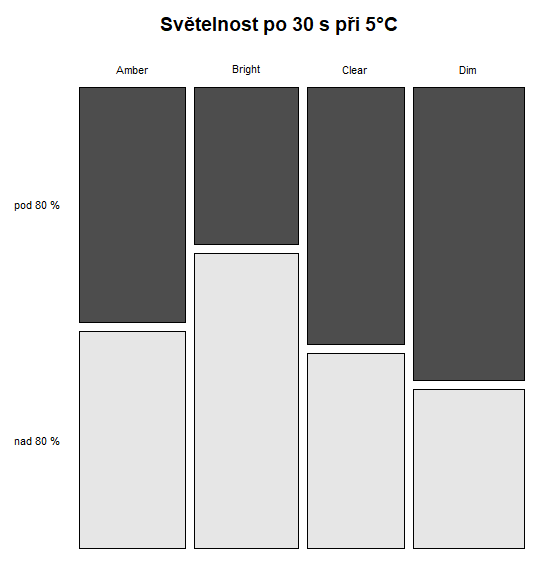
\includegraphics[width=0.6\textwidth]{Figures/Mosaic_4.png}
	\caption{Mozaikový graf dosažení 80\% světelnosti při 5°C, podle výrobce}
	\label{fig:Mosaic_4}
\end{figure}


% B)
\newpage
\subsection{}
V případě výrobce Bright určete bodový i 95\% intervalový odhad pravděpodobnosti, 
že při teplotě 5°C zářivka nedosáhne po 30 sekundách požadovaného světelného toku 
(80 \% deklarovaného maximálního světelného toku). 
Nezapomeňte na ověření předpokladů pro použití intervalového odhadu.

K nedosažení 80\% světelnosti u výrobce Bright došlo ve 24 (34,78 \%) případech.
Clopperův-Pearsonův intervalový odhad této pravděpodobnosti je (23,98;47,29) \%.
Předpoklad pro použití intervalového odhadu byly splněny ($9/(0,3478*0,6522)$ = 39,67 \textless{} 69)


% C)
\newpage
\subsection{}
Určete bodový i 95\% intervalový odhad relativního rizika, 
že zářivka při teplotě 5°C nedosáhne po 30 sekundách požadovaného světelného toku 
(80 \% deklarovaného maximálního světelného toku), pro „nejhoršího“ 
výrobce (vzhledem k „nejlepšímu“ výrobci). Výsledky slovně interpretujte.

Nejlepším výrobcem byl určen Bright a nejhorším Dim.
U výrobce Dim lze očekávat 1,86 krát vyšší riziko na nedosáhnutí 
80\% světelnosti zářivek než u výrobce Bright.
Dle 95\% intervalového odhadu lze toto relativní riziko očekávat v rozmezí (1,29;2,69).
Na základě intervalového odhadu lze konstatovat, že na hladině významnosti 0,05 lze 
vliv výrobce na výskyt nedosažení 80\% světelnosti považovat za závislý.


% D)
\newpage
\subsection{}
Určete bodový i 95\% intervalový odhad poměru šancí, 
že zářivka při teplotě 5°C nedosáhne po 30 sekundách požadovaného světelného toku 
(80 \% deklarovaného maximálního světelného toku), pro „nejhoršího“ výrobce 

(vzhledem k „nejlepšímu“ výrobci). Výsledky slovně interpretujte.

Nejlepší výrobce Bright má šanci na nedosažení 80\% světelnosti 533:1000, 
tj. na 1533 zářivek výrobce Bright lze očekávat 533 zářivek se světelností menší, než 80 \%.

Nejhorší výrobce Dim má šanci na nedosažení 80\% světelnosti 1846:1000, 
tj. na 2846 zářivek výrobce Bright lze očekávat 1846 zářivek se světelností menší, než 80 \%.

Z výše uvedeného je zřejmé, že u výrobce Dim je šance na menší než 80\% světelnost 3,46 krát vyšší
než u výrobce Bright. Dle 95\% intervalového odhadu lze tento poměr šancí očekávat v rozmezí
(1,73;6,89). Na základě intervalového odhadu lze konstatovat, že na hladině významnosti 0,05 lze
vliv výrobce na výskyt nedosažení požadovaného světelného toku považovat za závislý.


% E)
\newpage
\subsection{}
Pomocí chí-kvadrát testu nezávislosti rozhodněte, jestli to, 
že zářivka při teplotě 5°C nedosáhne po 30 sekundách požadovaného světelného toku 
(80 \% deklarovaného maximálního světelného toku), závisí statisticky významně 
na tom, od kterého výrobce zářivka pochází. Výsledky okomentujte.

Všechny očekávané četnosti jsou větší než 5, tj. pro ověření, 
zda po 30 sekundách zářivky nedosáhnou 80\% světelnosti při teplotě 5°C, 
statistiky významně závisí na tom, od kterého výrobce zářivky pochází, lze použít
$\chi^2$ test nezávislosti.

Výsledek $\chi^2$ testu nezávislosti (p-hodnota = 0,003) vypovídá o staticky významné 
závislosti mezi výrobcem zářivek a jejich schopností dosáhnout 80\% světelnosti.


\end{document}

